
\documentclass{article}
\usepackage{hyperref}
\usepackage{graphicx}
\usepackage{amsmath}
\usepackage{geometry}

\geometry{a4paper, margin=2.5cm}
\hypersetup{colorlinks=true, linkcolor=black}

\begin{document}
\sffamily
\large
\tableofcontents
\newpage

\section{How to}
\subsection{Adding, removing and changing channel numbers}
\subsubsection{Channel numbers}
Channel numbers are stored in \verb|main/channels.h|. Within the \verb|create_tv_channels()| function, a channel is
specified by writing \verb|CHANNEL("channel name", channel number);|. For example:
\begin{equation*}
    \verb|CHANNEL("BBC_ONE_HD", 101);|
\end{equation*}
The number can be changed without much issue, and the program will automatically figure out which number keys to press
on the remote when that channel is requested. The order of the channels does not matter here.

\begin{center}
    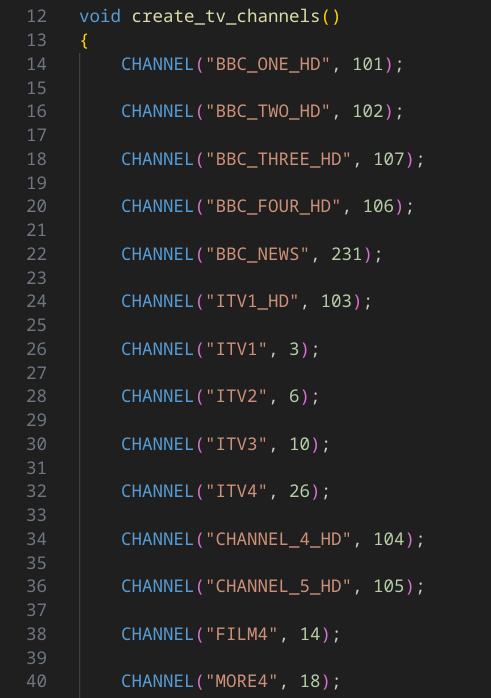
\includegraphics[width=0.8\textwidth]{images/example channels.png}
\end{center}

The name of the channel is important as this determines the name of the ``action list'' for that channel. In order to
allow each remote to send the numbers for a given channel, an action list for each remote is automatically created. The
names of the action lists are set by prefixing a name for the remote to the name of the channel. For example,
\verb|TV_BBC_ONE_HD| will be an action list of the TV remote's 1, 0 and 1 keys. \verb|HDR_BBC_ONE_HD| will be another
action list using the HDR remote's number keys instead. This prefixing can be seen in \verb|main/actionlist.h| in the
\verb|Channels| section.

Channels also need to be known by the UI so they can be used when generating the channel button grid. This is done in
\verb|main/ui/custom-component-data.slint|. In the \verb|ChannelButtonData| section, a list of channels is specified.
This list is used to create the buttons in the grid. \textbf{The order of this list is the order the buttons are created
in the grid, column by column.}

\begin{center}
    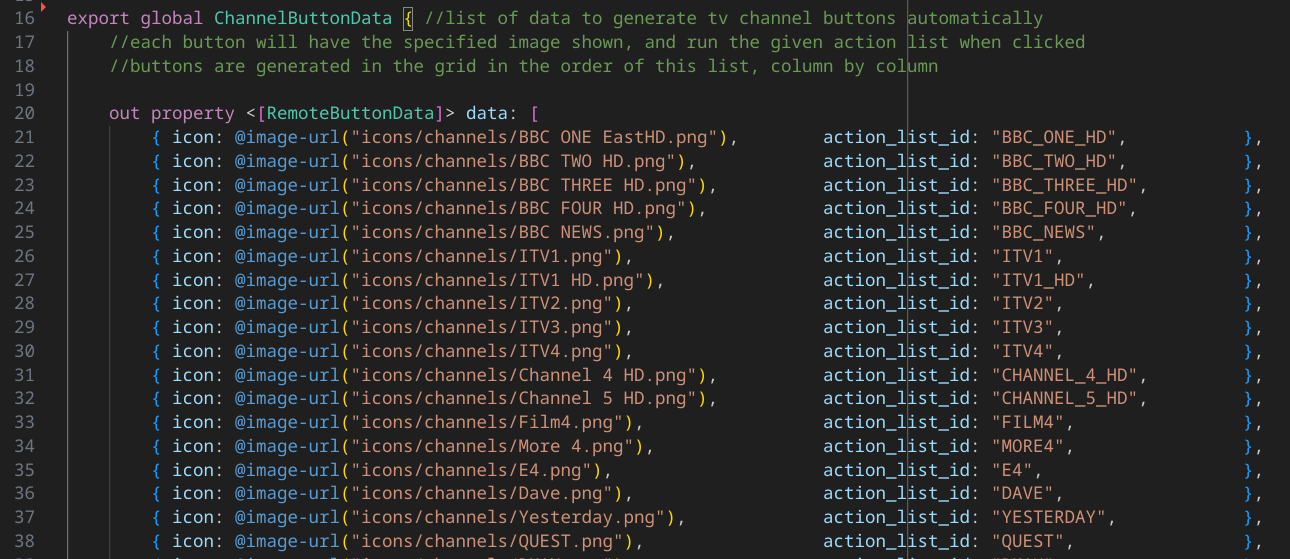
\includegraphics[width=\textwidth]{images/channel button data.png}
\end{center}

\subsubsection{Adding a new channel}
The full process for adding a new channel is as follows:
\begin{enumerate}
    \item Create a \verb|CHANNEL| in \verb|main/channels.h|
    \item Place the channel logo image in \verb|main/ui/icons/channels/|
    \item Add an entry in \verb|main/ui/custom-component-data.slint| in the \verb|ChannelButtonData| section
    \begin{itemize}
        \item The simplest way will be to copy an existing line (including both \{\} and the comma at the end)
        \item The \verb|icon| should be the directory to the channel image placed earlier. The directory is relative to
            the \verb|custom-component-data.slint| file, i.e. starting from the \verb|ui| folder.
        \item The \verb|action_list_id| should match the name used in \verb|CHANNEL(name, number)|
        \item The position of the entry will be where that channel is placed in the grid
    \end{itemize}
    \item The channel should now be added. \underline{\hyperref[secBuilding]{Build and upload the program to the remote}}.
\end{enumerate}

\subsubsection{Removing a channel}
The process for removing a channel is the reverse of adding one. The \verb|CHANNEL| in \verb|main/channels.h| should be
removed, as well as the entry in the list in \verb|main/ui/custom-component-data.slint|. Changing channel numbers only
needs requires editing \verb|channels.h|.

\subsection{Adding a new remote}
The learnt signals are stored in \verb|remotes.h| and organised per-remote. To add a new remote, first add a new
namespace in the file:
\begin{verbatim}
namespace NewRemoteName
{
    
}
\end{verbatim}
The codes for the remote will be placed in here. They are created by writing \verb|ACTION(name, "code")|. For example:
\begin{equation*}
    \verb|ACTION(POWER, "06e08da601b681b0052281b401bb81b101d4819...");|
\end{equation*}
The \verb|name| will be used later when referencing this \verb|action| in \verb|action lists|. The \verb|code| in the
example has been shortened, the actual code will be quite long.

\subsubsection{Learning signals}
To add codes to the new remote, first take the ESP remote and the original which is being learnt from. Connect the ESP
remote to the computer with USB. TODO: decide how to handle building/uploading/monitoring. most likely use WSL.

Navigate to the \verb|IR Recieve| screen in the ESP remote through the screen list:

\begin{center}
    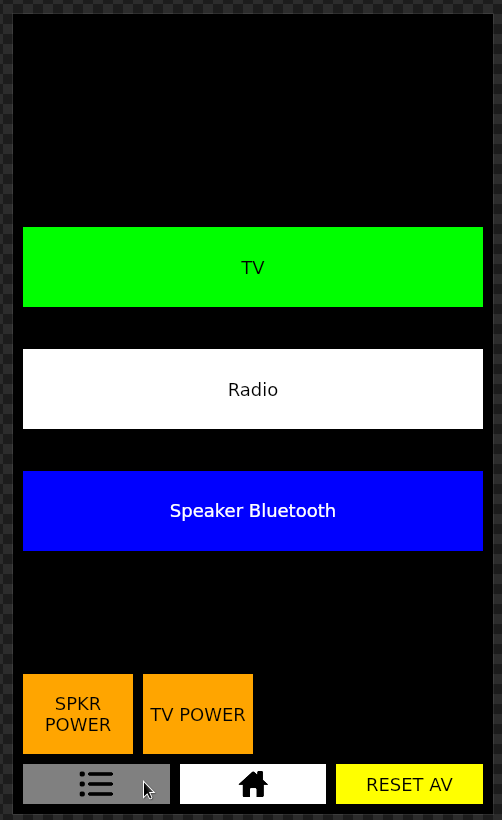
\includegraphics[width=0.32\textwidth]{images/ir learn 1.png}
    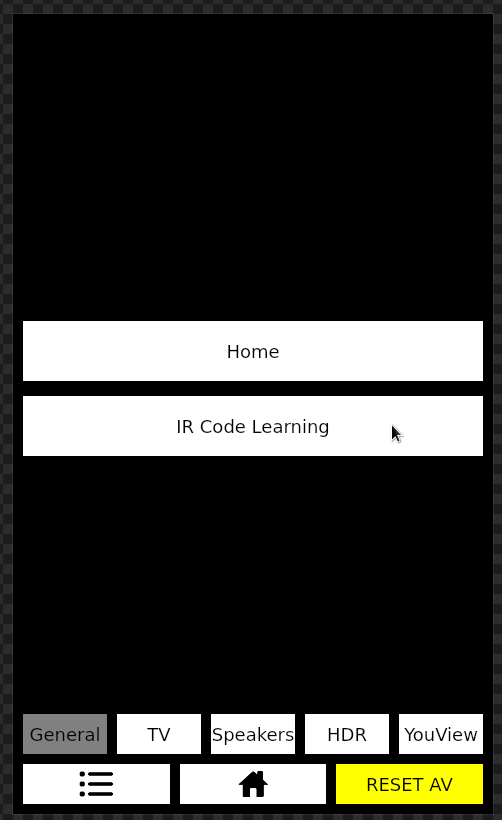
\includegraphics[width=0.32\textwidth]{images/ir learn 2.png}
    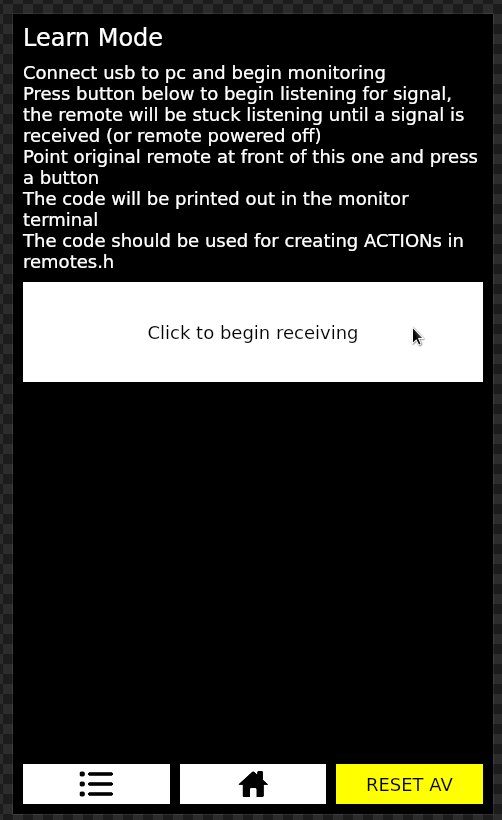
\includegraphics[width=0.32\textwidth]{images/ir learn 3.png}
\end{center}

Click the button to begin listening for a signal, then press a button on the remote being learnt. A code should appear
in the monitor terminal, highlight it and copy it.

Now go back to \verb|remotes.h| and create a new \verb|ACTION| with a suitable name, and paste the code between quote
marks. See the existing codes for examples. Repeat this for all the buttons on the remote.

\subsubsection{Creating action lists}
In order for a remote's signal to be used, it needs to be part of an \verb|action list|. An action list is a sequence of
one or more remote buttons which should be pressed automatically. These are created in \verb|main/actionlist.h|. The
action list file is organised with general macros at the top, followed by code for automatically generating channel
action lists, then by each remote's individual buttons. To simplify the program, all individual buttons still need to be
part of an \verb|action list|.

To create an \verb|action list| it needs to be added to the list of all action lists, appropriately named
\verb|ALL_ACTION_LISTS|. Within the function \verb|create_action_lists|, an action list is added to
\verb|ALL_ACTION_LISTS| with:
\begin{verbatim}
ALL_ACTION_LISTS["action list name"] = {
    RemoteName::ActionName,
    RemoteName::ActionName,
    ...
}
\end{verbatim}

\verb|RemoteName| is the namespace which the remote's \verb|ACTION| is in. 


\subsection{Building and uploading the program to the remote}\label{secBuilding}


\section{Documentation}
\subsection{Actions and action lists}
Based on the Phillips Pronto remotes, sending one or more IR signals is modeled with the concept of an \verb|Action|
which is a single IR signal akin to pressing a button on a remote, and an \verb|Action List| which is a sequence of
\verb|Actions|.

For extra functionality, there are currently 3 types of actions defined in \verb|main/action.h|:
\begin{itemize}
    \item \verb|ActionRemoteSignal| - a single signal from one learnt remote button press
    \item \verb|ActionDelayMilliseconds| - a delay of a given amount of time before the next \verb|action| is run
    \item \verb|ActionRepeatIRForMilliseconds| - a specified \verb|ActionRemoteSignal| is repeated quickly to mimic the
        button being held down for a given time period
\end{itemize}

\subsubsection{Creating actions}
The majority of actions are of type \verb|ActionRemoteSignal| learnt from a remote. These can be learnt through the
remote using the \verb|IR Receive| screen from the screens list in the \verb|general| tab.

The learnt signals are stored in \verb|main/remotes.h|. To easily support a variety of remotes, the signals are stored
as the series of high and low pair times which the ESP RMT peripheral understands. This means the codes are very long,
but no information needs to be stored about how the signal should be encoded, and signals from all remotes can be
treated the same way when learnt and sent.

A \verb|namespace| is created to separate each remote's \verb|actions|, and each \verb|action| is created with a macro
for simplicity:
\begin{equation*}
    \verb|ACTION(name, code)|
\end{equation*}
The \verb|name| argument is the variable name for the action in the remote namespace. The code is a string of the learnt
timing data for the signal.

\end{document}